% Five introduction slides; subsection entries create PDF navigation only.
% Project aims and architecture are proposed, not claims of completed hardware control.
\section{Introduction}
\subsection{Motivation and Context}

\begin{frame}[more-space]{Introduction\enspace|\enspace Motivation and Context}
  \begin{columns}[T,onlytextwidth]
    \column{0.31\textwidth}
      \datametric{7\,\% to $>30$\,\%}{Cooling share of facility electricity}
      \smallskip
      {\footnotesize Efficient hyperscale to less-efficient\\enterprise facilities; IEA estimates.}
    \column{0.65\textwidth}
      \dataheading{Cooling links energy, performance and reliability}
      More CPU power $\rightarrow$ more heat\\
      More cooling $\rightarrow$ additional electricity use\\
      Excess temperature $\rightarrow$ throttling and reliability risks
  \end{columns}

  \medskip
  \begin{columns}[T,onlytextwidth]
    \column{0.315\textwidth}
      \begin{beamercolorbox}[sep=2mm,wd=\linewidth]{data panel}
        \dataheading{Computing capacity}
        \footnotesize
        More available CPU power\\
        Within the thermal budget
      \end{beamercolorbox}
    \column{0.315\textwidth}
      \begin{beamercolorbox}[sep=2mm,wd=\linewidth]{data panel}
        \dataheading{Cooling efficiency}
        \footnotesize
        Penalize cooling effort\\
        Avoid unnecessary cooling
      \end{beamercolorbox}
    \column{0.315\textwidth}
      \begin{beamercolorbox}[sep=2mm,wd=\linewidth]{data panel}
        \dataheading{Thermal safety}
        \footnotesize
        Respect CPU temperature limits\\
        Account for predictive uncertainty
      \end{beamercolorbox}
  \end{columns}

  \medskip
  \begin{beamercolorbox}[sep=2mm,wd=\textwidth]{data panel}
    \dataheading{Project goal: safer and more efficient thermal management}
    Physics-informed, uncertainty-aware predictions\\
    $\longrightarrow$ operating decisions balancing compute, cooling and safety
  \end{beamercolorbox}

  \datasource{Context: \href{https://www.iea.org/reports/energy-and-ai/energy-demand-from-ai}{IEA, Energy and AI (2025), cooling electricity share by facility type}.
    Proposed objective: thermal management balancing computation, cooling and safety.}
\end{frame}

% Set the credit outside the frame body so the RWTH footer sees it.
% This group limits the extra footer text to the photo slide.
\begingroup
\footlinetext{\href{https://www.ri.se/en/news/from-idea-to-an-internationally-recognised-innovation-environment-ice-datacenter-celebrates}{Photo: RISE / ICE Datacenter (2026)}}
\begin{frame}[more-space]{Introduction\enspace|\enspace Motivation and Context}
  \begin{columns}[T,onlytextwidth]
    \column{0.50\textwidth}
      \dataheading{RISE ICE Datacenter / Lule\aa{}, Sweden}
      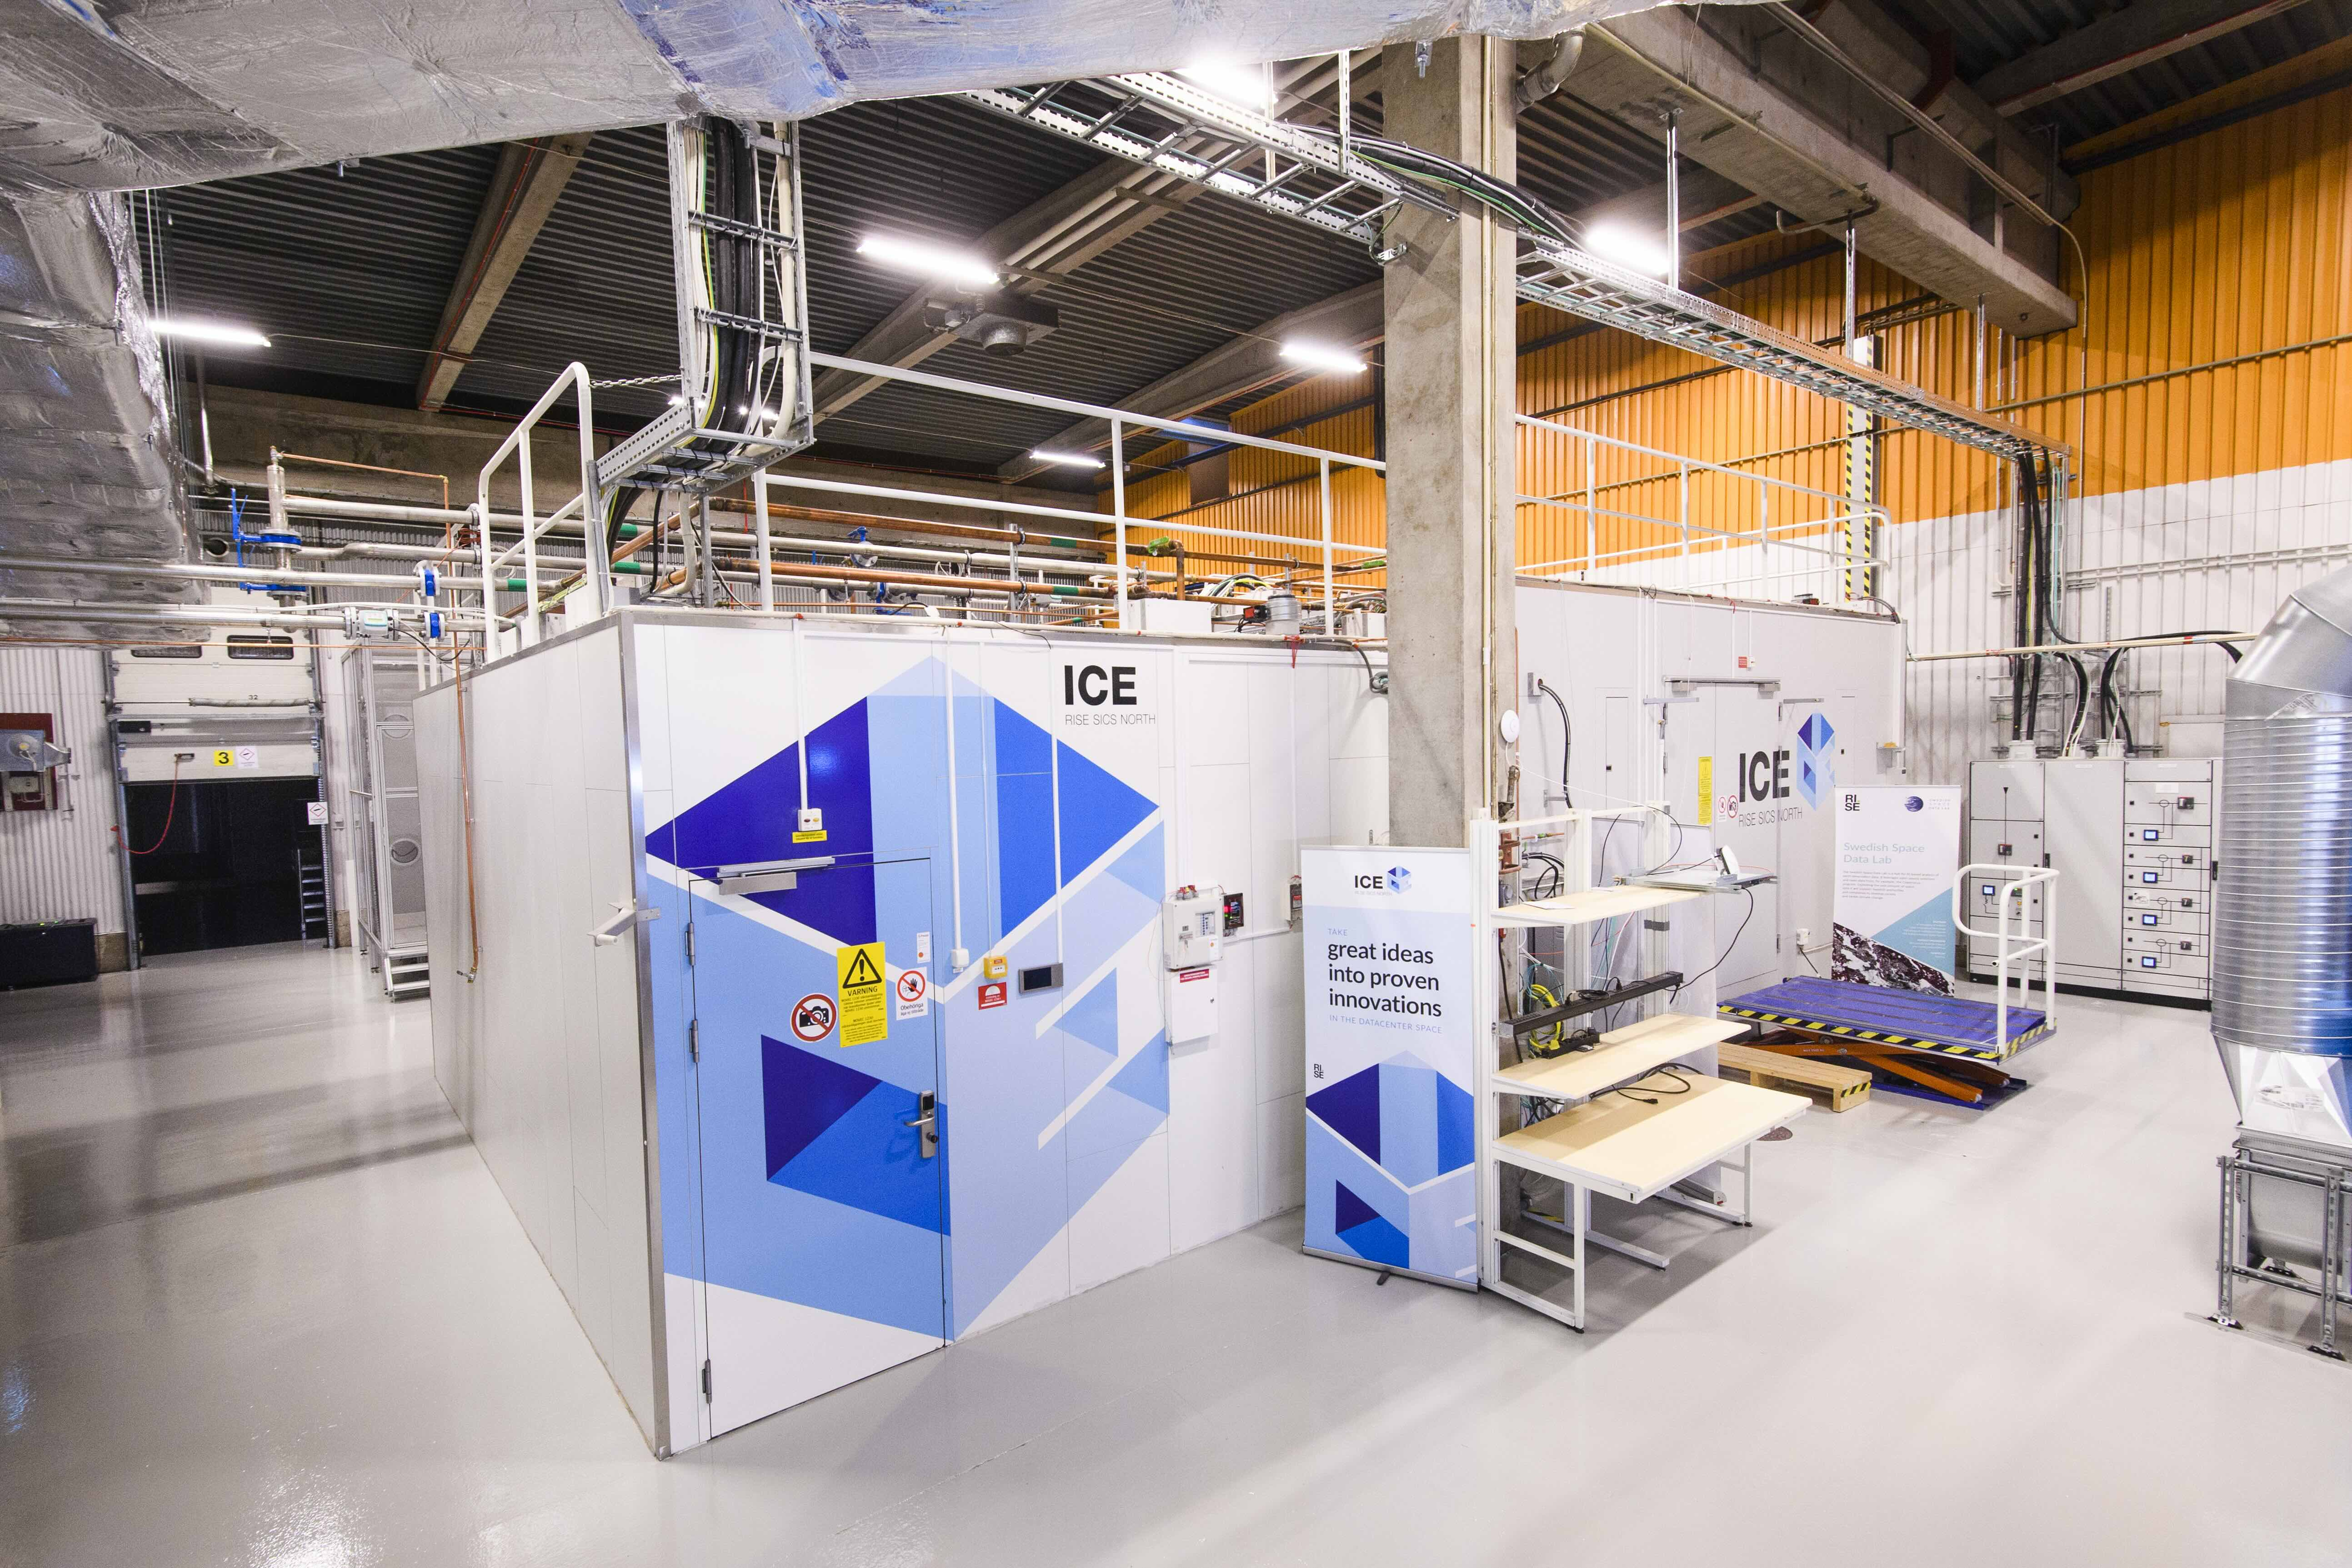
\includegraphics[width=\linewidth]{images/datacenter.jpeg}
    \column{0.46\textwidth}
      \dataheading{Experimental dataset}
      \textbf{9 OCP servers / 18 CPUs}\\
      Two Intel Xeon E5-2678 v3 CPUs per server\\
      Measurements in the RISE server wind tunnel

      \medskip
      \textbf{Original purpose}\\
      Air vs. two-phase direct-to-chip cooling\\
      Thermal performance / energy / throttling

  \end{columns}

  \datasource{Dataset: \href{https://doi.org/10.5281/zenodo.23237930}{HEATWISE / Zenodo 23237930};
    \href{https://doi.org/10.1016/j.csite.2026.107650}{Ebrahimpour Ahmadi et al., CSITE 78 (2026), 107650}.}
\end{frame}
\endgroup

\begin{frame}[more-space]{Introduction\enspace|\enspace Our Goal: An Air-cooling Actuator Digital Twin}
  \begin{columns}[T,onlytextwidth]
    \column{0.32\textwidth}
      \begin{beamercolorbox}[sep=2mm,wd=\linewidth]{data panel}
        \dataheading{Air-cooling subset}
        \textbf{1,333 records / 219 variables}\\
        \footnotesize
        Five-minute values\\
        31 Oct--5 Nov 2024

        \medskip
        \textbf{Cases 1--5}\\
        Hybrid cases excluded
      \end{beamercolorbox}

    \column{0.64\textwidth}
      \dataheading{Goal: maximize CPU power within a temperature limit}
      Optimal CPU-power and fan-power control inputs

      \medskip
      {\footnotesize
      \renewcommand{\arraystretch}{1.2}
      \begin{tabular*}{\linewidth}{@{\extracolsep{\fill}}ll@{}}
        \toprule
        \textbf{Target controls} & CPU power $P_{\mathrm{CPU}}$ / fan power $P_{\mathrm{fan}}$\\
        \textbf{Given condition} & Cooling-air inlet temperature $T_{\mathrm{in}}$\\
        \textbf{Twin prediction} & Maximum steady-state CPU temperature\\
        \bottomrule
      \end{tabular*}
      }

      \medskip
      \begin{beamercolorbox}[sep=2mm,wd=\linewidth]{data panel}
        \dataheading{Thermal constraint}
        $\widehat{T}_{\max}^{\mathrm{ss}}(P_{\mathrm{CPU}},T_{\mathrm{in}},P_{\mathrm{fan}})
          + \Delta_{\mathrm{UQ}} \leq T_{\mathrm{limit}}$
        \par\smallskip
        \footnotesize
        Predictive uncertainty margin / actuator bounds
      \end{beamercolorbox}
  \end{columns}

  \medskip
  \begin{beamercolorbox}[sep=2mm,wd=\textwidth]{data panel}
    \footnotesize
    \textbf{Computing capacity}\quad Maximize available CPU power without exceeding the thermal limit\\
    \textbf{Cooling efficiency}\quad Penalize cooling effort when selecting feasible operating points
  \end{beamercolorbox}

  \datasource{Proposed offline optimization; live actuation conceptual.
    Current data: raw fan signal with unverified unit; physical fan-power calibration required.
    Subset: dataset README and exploratory audit.}
\end{frame}

\subsection{Why a Digital Twin?}

\begin{frame}[more-space]{Introduction\enspace|\enspace Why a Digital Twin?}
  \dataheading{A measured system linked to predictions and operating decisions}
  \begin{center}
    \begin{tikzpicture}[
      node distance=5mm,
      stage/.style={fill=rwth-blue-100!6,inner sep=2mm,text width=39mm,
        minimum height=19mm,align=left,font=\footnotesize},
      >={Latex[length=2mm]}
    ]
      \node[stage] (measurements) {\textbf{Server measurements}\\
        CPU power / inlet temperature\\
        Raw fan signal\\
        Steady-state observations};
      \node[stage,right=of measurements] (surrogate) {\textbf{Proposed PI-PCE surrogate}\\
        Steady-state CPU $T_{\max}$\\
        Thermal-resistance loss\\
        Uncertainty + Sobol analysis};
      \node[stage,right=of surrogate] (decisions) {\textbf{Constrained decisions}\\
        CPU power vs. cooling effort\\
        Thermal + actuator limits\\
        Uncertainty-aware optimization};
      \draw[->,thick,rwth-blue-100] (measurements) -- (surrogate);
      \draw[->,thick,rwth-blue-100] (surrogate) -- (decisions);
    \end{tikzpicture}
  \end{center}

  \smallskip
  \begin{columns}[T,onlytextwidth]
    \column{0.315\textwidth}
      \dataheading{Fast optimization / control loop}
      \footnotesize
      Rapid surrogate evaluations\\
      Candidate operating setpoints
    \column{0.315\textwidth}
      \dataheading{Independent thermal safety}
      \footnotesize
      Measured-temperature checks\\
      Override / safe fallback actions
    \column{0.315\textwidth}
      \dataheading{Slower model-updating loop}
      \footnotesize
      New steady-state measurements\\
      Surrogate updates + revalidation
  \end{columns}

  \medskip
  \begin{beamercolorbox}[sep=2mm,wd=\textwidth]{data warning}
    \footnotesize
    \textbf{Scope}\quad Offline analysis, surrogate development, validation, UQ, sensitivity and optimization\\
    \textbf{Live hardware control}\quad Conceptual architecture; no experimental control demonstration
  \end{beamercolorbox}

  \datasource{Proposed project architecture. PCE = Polynomial Chaos Expansion;
    UQ = uncertainty quantification; Sobol analysis = variance-based input sensitivity.
    Cooling input retained as a raw signal until its unit is verified.}
\end{frame}

\subsection{Why not Synthetic Data?}

\begin{frame}[more-space]{Introduction\enspace|\enspace Why not Synthetic Data?}
  \dataheading{Project choice: anchor the model in measured server behavior}
  \begin{columns}[T,onlytextwidth]
    \column{0.48\textwidth}
      \begin{beamercolorbox}[sep=2.5mm,wd=\linewidth]{data warning}
        \dataheading{Training on simulator-generated targets}
        \textbf{Assumptions become the training reference}\\
        \footnotesize
        Thermal parameters / cooling boundary conditions\\
        Fan calibration / sensor and model discrepancy

        \medskip
        \textbf{More samples, same potential model bias}\\
        Simulator-only validation: limited hardware evidence
      \end{beamercolorbox}

    \column{0.48\textwidth}
      \begin{beamercolorbox}[sep=2.5mm,wd=\linewidth]{data panel}
        \dataheading{Experimental measurements + physics}
        \textbf{Observed response of the real servers}\\
        \footnotesize
        Load changes / cooling interactions / variability\\
        Independent measurement-based validation

        \medskip
        \textbf{Physics as guidance for the PCE}\\
        Thermal-resistance loss for plausible predictions
      \end{beamercolorbox}
  \end{columns}

  \medskip
  \begin{beamercolorbox}[sep=2mm,wd=\textwidth]{data panel}
    \dataheading{A supplementary role for synthetic data}
    \footnotesize
    Calibrated, validated simulators $\rightarrow$ augmentation and scenario tests\\
    Hardware evidence remains essential for thermal-safety validation
  \end{beamercolorbox}

  \medskip
  {\footnotesize\textbf{Next:} experimental coverage, measurement limitations and steady-state selection.}

  \datasource{Project rationale. Experimental-data constraints: dataset README, DATA\_DICTIONARY.csv and exploratory audit.
    Training and validation strategy: proposed project work.}
\end{frame}
